% -*- root: Document.tex -*-

\chapter{Background}
\label{chap:background}

The design of \SS{} revolves around the availability of SGX features in the host machines.
It consists in a \emph{trusted execution environment} (TEE) recently introduced into Intel{\textregistered} SkyLake, similar in spirit to ARM \textsc{TrustZone}~\cite{arm2009security} but much more powerful.
Applications create secure \emph{enclaves} to protect the integrity and the confidentiality of the data and the code being executed.

The SGX mechanism, as depicted in Figure~\ref{fig:sgx}, allows applications to access confidential data from inside the enclave.
The architecture guarantees that an attacker with physical access to a machine will not be able to tamper with the application data without being noticed.
The CPU package represents the security boundary.
Moreover, data belonging to an enclave is automatically encrypted and authenticated when stored in main memory.
A memory dump on a victim's machine will produce encrypted data.
A \emph{remote attestation protocol} allows one to verify that an enclave runs on a genuine Intel{\textregistered} processor with SGX.
An application using enclaves must ship a signed (not encrypted) shared library (a shared object file in Linux) that can possibly be inspected by malicious attackers.

In the current version of SGX, the \emph{enclave page cache} (EPC) is a $128\,\mathit{MB}$ area of memory\footnote{Future releases of SGX might relax this limitation~\cite{mckeen2016intel}.} predefined at boot to store enclaved code and data.
At most around $90\,\mathit{MB}$ can be used by application's memory pages, while the remaining area is used to maintain SGX metadata.
Any access to an enclave page that does not reside in the EPC triggers a page fault.
The SGX driver interacts with the CPU to choose which pages to evict.
The traffic between the CPU and the system memory is kept confidential by the \emph{memory encryption engine} (MEE)~\cite{gueron2016memory}, also in charge of tamper resistance and replay protection.
If a cache miss hits a protected region, the MEE encrypts or decrypts data before sending to, respectively fetching from, the system memory and performs integrity checks.
Data can also be persisted on stable storage protected by a seal key.
This allows the storage of certificates, waiving the need of a new remote attestation every time an enclave application restarts.

\begin{figure}[H]
  \centering
  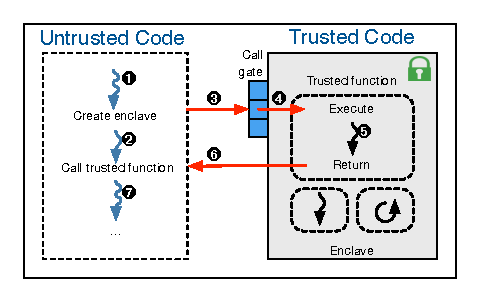
\includegraphics[width=0.65\linewidth]{Figures/sgx}
  \caption{SGX core operating principles.}
  \label{fig:sgx}
\end{figure}

The execution flow of a program using SGX enclaves is like the following.
First, an enclave is created (see Figure~\ref{fig:sgx}-\ding{202}).
As soon as a program needs to execute a trusted function (\ding{203}), it executes SGX's primitive \texttt{ecall} (\ding{204}).
The call goes through the SGX call gate to bring the execution flow inside the enclave (\ding{205}).
Once the trusted function is executed by one of the enclave's threads (\ding{206}), its result is encrypted and sent back (\ding{207}) before giving back the control to the main processing thread (\ding{208}).
